%%%%%%%%%%%%%%%%%%%%%%%%%%%%%%%%%%%%%%%%%%%%%%%%%%%%%%%%%%%%%%%%%%%%%%%%%%%%%%%%
%2345678901234567890123456789012345678901234567890123456789012345678901234567890
%        1         2         3         4         5         6         7         8

\documentclass[letterpaper, 10 pt, conference]{ieeeconf}  % Comment this line out if you need a4paper

%\documentclass[a4paper, 10pt, conference]{ieeeconf}      % Use this line for a4 paper

\IEEEoverridecommandlockouts                              % This command is only needed if 
                                                          % you want to use the \thanks command

\overrideIEEEmargins                                      % Needed to meet printer requirements.

%In case you encounter the following error:
%Error 1010 The PDF file may be corrupt (unable to open PDF file) OR
%Error 1000 An error occurred while parsing a contents stream. Unable to analyze the PDF file.
%This is a known problem with pdfLaTeX conversion filter. The file cannot be opened with acrobat reader
%Please use one of the alternatives below to circumvent this error by uncommenting one or the other
%\pdfobjcompresslevel=0
%\pdfminorversion=4

% See the \addtolength command later in the file to balance the column lengths
% on the last page of the document

% The following packages can be found on http:\\www.ctan.org
%\usepackage{graphics} % for pdf, bitmapped graphics files
%\usepackage{epsfig} % for postscript graphics files
%\usepackage{mathptmx} % assumes new font selection scheme installed
%\usepackage{times} % assumes new font selection scheme installed
%\usepackage{amsmath} % assumes amsmath package installed
%\usepackage{amssymb}  % assumes amsmath package installed

\usepackage{tabularx}
\usepackage{color, colortbl}
\definecolor{Gray}{gray}{0.7}

\title{\LARGE \bf
To signal or not to signal: the question is what should a robot convey
}


\author{Hooman Hedayati$^{1}$ and Daniel Szafir$^{2}$% <-this % stops a space
\thanks{$^{1}$Department of Computer Science, University of Colorado Boulder.
        {\tt\small hooman.hedayati@colorado.edu}}%
	\thanks{$^{2}$Department of Computer Science and ATLAS Institute, University of Colorado Boulder.
		{\tt\small daniel.szafir@colorado.edu}}%
}


\begin{document}



\maketitle
\thispagestyle{empty}
\pagestyle{empty}


%%%%%%%%%%%%%%%%%%%%%%%%%%%%%%%%%%%%%%%%%%%%%%%%%%%%%%%%%%%%%%%%%%%%%%%%%%%%%%%%
\begin{abstract}
With the advance in technology, robots are used in more than any time. Robots are becoming an essential part of factories, homes, etc. Although some of them are behind cages, most of them are exposed to human. As a result, the number of interactions between human and robots increasing rapidly. For better interaction, both robot and human should have some fundamental knowledge about each other, this knowledge is a key to safe, appealing, etc., human-robot interaction e.g., with the signal a pedestrian knows where the self-driving car going toward. In this paper, we explore the type of information that robots should convey to the users.  We made videos of a user interacting with 3 different robots, a small size ground robot, a big size ground robot with manipulator and an aerial robot and created a "priority list" consist of possible information a user might want to know and designed a survey in which participants must select what type of information they want to know. We recruited 150 participants on Mechanical Turk and share our finding as a list of the user's priorities in the result section.

\end{abstract}


%%%%%%%%%%%%%%%%%%%%%%%%%%%%%%%%%%%%%%%%%%%%%%%%%%%%%%%%%%%%%%%%%%%%%%%%%%%%%%%%
\section{INTRODUCTION}
In the last few years with the advances in technology, robots are used more than anytime and this is still growing.
\begin{itemize}
\item Aerial robots: are going to be used for to go were a users can't go e.g., bridge inspection \cite{chan2015towards}, help astronauts on the international space station (ISS)\cite{bualat2015astrobee}, for package delivery \cite{d2014guest}, etc. 
\item Other than traditional industrial robots which only exists in cages, there are new mobile industrial robots which move around the factories and warehouses and perform a variety of tasks such as moving payload or shelves \cite{wurman2008coordinating}. Some of these mobile base robots have a manipulator and can perform a manipulation task \cite{datta2008development, hvilshoj2011little}. 

\item Service robots are the other emerging group. The main goal of service robots is to assist humans in a non-industrial environment such as customers service related task (e.g., welcoming, guiding, taking orders, delivering, etc.) in shopping centers, restaurants, hotels, etc. \cite{acosta2006design, datta2011pilot, kanda2009affective, osawa2017real, zalama2014sacarino}. or cleaning and vacuuming the houses\cite{forlizzi2006service}.

\end{itemize}

The mentioned groups of robots have something in common. They mostly operate in a shared space with human or they teleoperate by a human. As a result of increase in number of robots, the number of interactions with human increase too. This interactions can be coexistence, coordination or collaboration \cite{cha2018survey}. A significant amount of research has been done in the field of human-robot interaction (HRI) \cite{goodrich2008human}. The ultimate goal is to design a robot in which people have a smooth, safe, enjoyable, productive, etc. interaction with. This might not possible without communicating and collaborating with the human \cite{cha2018survey, khatib1999robots}. 

In a human-human interaction, people are good at interpreting the signals coming from the opponent e.g., if two people passing by each other in a narrow hallway, often they are good at signaling/interpreting signal which path ( right or left ) are they going to take. If they can not perform a good job, the mentioned interaction would become an awkward situation. For a good interaction, both human and robot should have a basic understanding of each other. It is essential for a human to know more about the state of the robot and it is necessary for the robot to convey needed information to the user.

There is a large amount of literature about human's mental model \cite{aggarwal2011human}, the works that have been done to convey specific information \cite{ arras2005we, bauer2008human} and what signals to use to convey specific information\cite{cha2018survey}. As an example to convey "where the robot is moving next", Szafir et al. used gaze and lights \cite{szafir2015communicating}, Walker et al, used Augmented reality \cite{walker2018communicating}, Cha et al, used sound \cite{cha2018effects}. 

In this paper instead of "what medium to signal specific information?" , we are curious about "what information should the robot conveys?". This is an important question for designers/researchers to keep in mind while making a robot. Other than specific use cases e.g., designing the bomb difusal robot \cite{adams2005human}, to best our knowledge no one asked what type of information users needed to know about the robot.

We recruited 150 participants in 3 groups on Mechanical Turk and each group which consisted of 50 participants see one of the three different robots. 1) An aerial robot 2) A small ground robot which is in the similar size of small service robot and an industrial robot. 3) A large ground robot with a manipulator which is a similar size of a mobile industrial robot and service robot. We asked them about the information they want to know about the robot and we would share our finding in the result section.

\section{survey and procedure}
    We designed a survey with 4 sections. In the first section, participants watched two short videos, each approximately 30 seconds in duration. Both videos depicted a user completing a pick-and-place task while sharing an environment with one of 3 robots (Figure \ref{fig:task}). There are two tables in the environment. One table contains the user instructions and two boxes, while the other table contains various wooden blocks with associated numbers. The instructions required the user to follow a sequence of steps in which they selected a specified block from one table and placed it in one of the boxes in the other table (e.g., "1. The yellow pyramid with number 15 should go in Box A"). 
    
    In both videos, the robot acted as a supervisor, which meant that it occasionally went close to the tables and checked the current status of the task (e.g., how many objects were in a box or whether objects were placed in the correct box). In the first video, the robot was on the opposite side of the table and completely isolated from the user (Figure \ref{fig:task} top left). However, in the second video, the robot went the same side of the table as the user and thus at times was in the way of the path that the user tried to take (Figure \ref{fig:task} top right). Our goal in designing these two videos was to highlight scenarios in which users may simply coexist in shared environments with robots (i.e., bystander interaction) as well as scenarios requiring more direct interaction (e.g., to resolve right-of-way issues) as the information that users desire from the robot may depend on the amount and type of interaction. %We designed the videos to mimic two scenarios, in the first one the user and aerial robot are just in the same space there is not any interaction between them, but at the same time there couple of question that the user might want to know about the robot. In the second video, there is actually an interaction between them, the robot is on the way of the user and in this case.
    
    \begin{figure*}[h]
    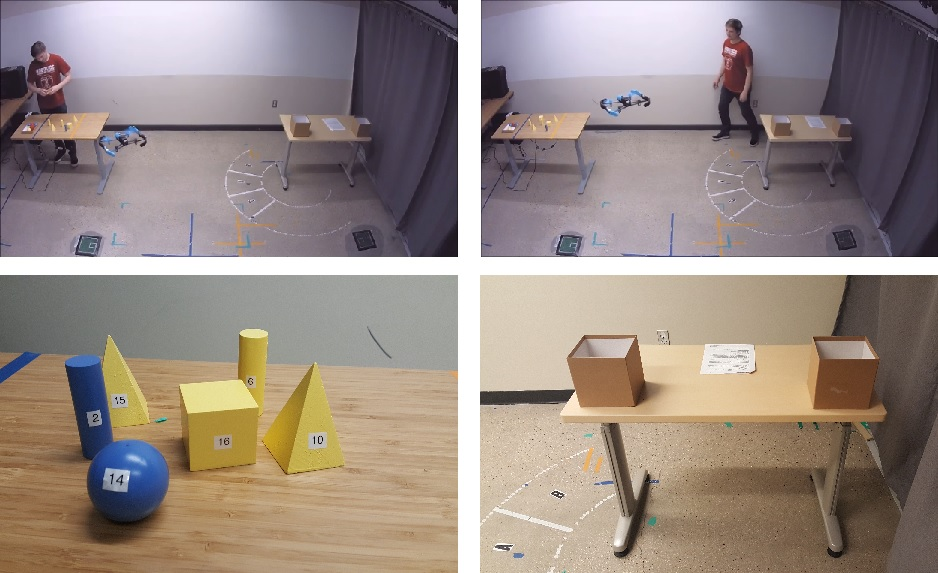
\includegraphics[width=\textwidth,height=15cm]{task.jpg}
    \caption{Top left: The robot doing a supervisory task. Top right: The robot intentionally interferes with the path the user is taking. Bottom: Pick and place task that the user is performing in the videos.}
    \label{fig:task}
    \end{figure*}
    
    After watching the videos (participants could re-watch videos at anytime of the survey), participants ranked number of items (22 items for the aerial robot and 21 items for the ground robots, the items are almost the similar expect for the "The robot conveying when it will change its altitude." which dose not applicable for ground robots), each of which corresponded to some sort of information that the robot might convey, in order of how important the participant perceived this information to be were they to interact with a robot as in the videos they had just watched. These items were drawn from a list of possible information that users might want to know from the robot created by reviewing prior HRI literature and a series of brainstorming sessions with expert roboticists with at least 5 years of experience (table \ref{table:list} in appendix A). 
    
    We can roughly categorize the items in 3 major groups. First \textit{condition}\cite{cha2018survey}, several items correspond to various information the robot might convey about itself, such as ``The robot conveying whether or not its camera is recording'' or ``The robot conveying when and in what direction robot would move next'' etc. The second group (\textit{activity}\cite{cha2018survey}) represents information that the robot might convey about the task it is doing, for example ``The robot conveying a list of successfully/unsuccessfully completed tasks (task history)'' or ``The robot conveying whether or not any faults/errors are detected (e.g., electric circuits damaged, payloads/sensors not mounted correctly, etc.).'' Finally, the third group corresponds with information related to whether it is safe and/or appropriate for human interaction, such as ``The robot conveying whether or not it is safe to get close to it'' or ``The robot conveying whether or not it currently knows where you are.'' For each participant, the list of items was presented to participants randomized in order to reduce the potential for initial placement bias. Participants were tasked with re-ordering the list of items in order of their perceived priority. 
    
    In the next section, participants were asked to provide a 1--7 Likert-type rating regarding their perceived importance for each item they ranked in the previous section. Here 1 was defined as ``not important'' and 7 was defined as ``very important.'' This section of the survey served two primary purposes. First, this section helped provide supplementary information on perceptions of absolute importance to contextualize the information on relative importance from the previous section (e.g., even items ordered near the end might be perceived as highly important by participants). Second, these questions provided a validation method for the items in the previous section (i.e., items ranked lower in the prior section should also receive an equal or lower score in this section). This validation helped us identify and control for the quality of participant responses. %Although it might seem like an unnecessary and redundant question, it is really important as a validation method. Using ranking question with more than 5 items is not suggested as people might not remember all the items in the list. In these cases the first and the last couple of items in the ranking are reliable, but the data in the middle might be noisy as a result not remembering the whole list. Since our list for ranking has more than 5 items, we used the second question for validation. The answers to the ranking question should have the same trend as the second question does. As an example, if the first item on the ranking should have higher or at least the equal as compare to the last item in the ranking answer. This help to remove the answers which are not consistent.

    While we created a large sample of items corresponding to different types of information it may be useful for a robot to convey, we recognize that our list is not exhaustive and might be missing potentially critical aspects. As a result, the next section of the survey provided participants with open-ended questions where participants could suggest any other information they think would be helpful to know about the robot or useful for the robot communicate to them. For each suggestion, we also asked participants to provide a Likert-type rating of 1--7 regarding how important they believe this suggested information might be. Each participant had the option to provide and rate 3 new suggestions. %The question asked to give us a better understanding of what a user wants and how important is that feature for that user. 

    In the last section of the survey, we collected demographic information regarding age, gender, education and the level of familiarity of participants with robots in general. We also included a question about obvious features in the two videos, in this case we asked the number of boxes on the table in order to ensure that participants actually watched the videos.

    With IRB approval we deployed the survey on Amazon Mechanical Turk and collected responses from 186 participants. After initial validation analysis, we removed data from 36 participants who didn't pass the video sanity check or  with inconsistencies across the ranking and rating sections. %Which mean their first item in ranking question has a lower likert score in the second question than their last item in the ranking. e.g., one participant's first rank is "The robot conveying whether or not there is a problem with the engines/motors." with 4 as a score, and the last item in the ranking is  "The robot conveying the current time and date." with 6 as a score. 
    As a result, we ended up with 150 responses for full analysis.

\section{result and finding}

    Among valid responses,10 participants identified themselves as female while 27 identified as male. Average participant age was 33.2 (SD = 8.4), with a range of 22 - 59. On a seven-point scale, participants reported a moderate prior familiarity with both aerial robots (M = 4.0, SD = 1.4). For each item on the priority list, the average score of responses calculated with a range of 7.9 - 16.8. In which, 1 means it's on user's top choice and 22 means the item is user's last choice. Using ranking question with more than 5 items is not suggested as people might not remember all the items in the list. In these cases the first and the last couple of items in the ranking are reliable, but the data in the middle might be noisy as a result not remembering the whole list. The average scores sorted. While the difference between the two consecutive item's score is almost continuous (M=0.32), two gaps were observed. From the 6th item to 7th, which the difference is 0.97 and between 19th and 20th which the difference is 1.79. We believe these two gaps dived the most important information and also the least important information as follow:



This is pretty interesting that the area which is on top users rank is not well explored. We are interested to explore those in our future work.

\subsection{Aerial Robot}

\begin {table}
\begin{center}
\label{table:bebop}
\begin{tabular}{|c|p{160pt}|c|c|}
 \hline
 \multicolumn{4}{|c|}{Most important} \\
 \hline
 Rank & The robot conveying ... & Mean & SD \\
 \hline
 \rowcolor{Gray}
 1 & whether or not it is safe to get close to it. & 8.0 & 5.2\\
 \hline
 \rowcolor{Gray}
2 & whether it is currently acting autonomously or being controlled by a person. & 8.3 & 6.1\\
 \hline
 \rowcolor{Gray}
3 & what it knows about the surrounding environment. & 8.8 & 4.3\\
 \hline
4 & whether or not any faults/errors are detected. & 9.6 & 5.8\\
 \hline
5 & when and in what direction robot would move next. & 9.7 & 5.7\\
 \hline
\end{tabular}

\vspace*{0.5 cm}

\begin{tabular}{|c|p{160pt}|c|c|}
 \hline
  \multicolumn{4}{|c|}{Least important} \\
 \hline
 Rank & The robot conveying ... & Mean & SD \\
 \hline
18 & its most recent maintenance report. & 13.9 & 5.5 \\
 \hline
19 & its total flight duration. & 13.9 & 5.7 \\
 \hline
 \rowcolor{Gray}
20 & how to look up more information about the robot. & 15.5 & 6.4 \\
 \hline
 \rowcolor{Gray}
21 & the current time and date. & 15.9 & 6.1 \\
 \hline
 \rowcolor{Gray}
22 & contact information for how to leave feedback about the robot. & 15.9 & 6.8 \\
 \hline
 
\end{tabular}
\end{center}

\caption{List of the most important items based on participants ranking for aerial robot}
\end{table}







\subsection{Small ground robot}


\begin {table}
\begin{center}
\label{table:turtlebot}
\begin{tabular}{|c|p{160pt}|c|c|}
 \hline
 \multicolumn{4}{|c|}{Most important} \\
 \hline
  Rank & The robot conveying ... & Mean & SD \\
 \hline
 \rowcolor{Gray}
1 & whether or not it is safe to get close to it. & 5.5 & 5.2\\
\hline
2 & when and in what direction robot would move next. & 8.3 & 6\\
\hline
3 & its current task progress (as a percentage of the whole task). & 8.3 & 4.5\\
\hline
4 & whether or not it needs assistance. & 8.8 & 5.7\\
\hline
5 & whether it is currently acting autonomously or being controlled by a person. & 8.9 & 5.8\\
\hline
\end{tabular}

\vspace*{0.5 cm}

\begin{tabular}{|c|p{160pt}|c|c|}
 \hline
  \multicolumn{4}{|c|}{Least important} \\
 \hline
  Rank & The robot conveying ... & Mean & SD \\
 \hline
    \rowcolor{Gray}
17 & The robot conveying its wireless signal strength. & 14.2 & 4.7\\
\hline
   \rowcolor{Gray}
18 & how to look up more information about the robot. & 14.3 & 5.7\\
\hline
   \rowcolor{Gray}
19 & the current time and date. & 14.9 & 5.6\\
\hline
   \rowcolor{Gray}
20 & its remaining battery life as a percentage. & 15.4 & 5.1\\
\hline
   \rowcolor{Gray}
21 & contact information for how to leave feedback about the robot. & 15.7 & 4.9\\
\hline
\end{tabular}
\end{center}

\caption{List of the most important items based on participants ranking for small ground robot}
\end{table}





\subsection{Large ground robot}


\begin {table}
\begin{center}
\label{table:fetch}
\begin{tabular}{|c|p{160pt}|c|c|}
 \hline
 \multicolumn{4}{|c|}{Most important} \\
 \hline
  Rank & The robot conveying ... & Mean & SD \\
 \hline
   \rowcolor{Gray}
1 & whether or not it is safe to get close to it. & 7.2 & 6.1\\
 \hline
2 & when and in what direction robot would move next. & 8.1 & 5.5\\
 \hline
3 & whether or not it needs assistance. & 8.3 & 5.6\\
 \hline
4 & whether or not it currently knows where you are. & 8.3 & 5.4\\
 \hline
5 & whether or not its camera is recording. & 9.1 & 4.1\\
 \hline
\end{tabular}

\vspace*{0.5 cm}

\begin{tabular}{|c|p{160pt}|c|c|}
 \hline
  \multicolumn{4}{|c|}{Least important} \\
 \hline
  Rank & The robot conveying ... & Mean & SD \\
 \hline
 
   \rowcolor{Gray}
17 & how to look up more information about the robot. & 13.8 & 4.9\\
\hline
   \rowcolor{Gray}
18 & The robot conveying its remaining battery life as a percentage. & 14 & 5.8\\
\hline
   \rowcolor{Gray}
19 & The robot conveying its most recent maintenance report. & 14 & 5.3\\
\hline
   \rowcolor{Gray}
20 & The robot conveying the current time and date. & 14.8 & 5.3\\
\hline
   \rowcolor{Gray}
21 & The robot conveying contact information for how to leave feedback about the robot. & 16.4 & 4.8\\
\hline
\end{tabular}
\end{center}

\caption{List of the most important items based on participants ranking for Large ground robot}
\end{table}



For the open-ended questions, 45 answered received from 28 participants (M = 1.21). 17 participants provided a suggestion, 5 provided two suggestions and 6 participants provided 3 suggestions. After reviewing the data and removing the ones which were similar to one of the items in the priority list, we find 4 new categories. There is a set of suggestions which wanted to know about the environment in which the robot is working: 
\begin{itemize}
    \item  \textbf{Participant 15, importance 2:} "Rain or Water alert"
    \item  \textbf{Participant 20, importance 5:} "Whether it is entering a restricted area."
    \item  \textbf{Participant 15, importance 3:} "Heavy Wind alert"
\end{itemize}



The second group is the information about the safely of robot itself:
\begin{itemize}
    \item  \textbf{Participant 24, importance 3:} "How close the robot is from touching the floor or the ceiling"
    \item  \textbf{Participant 4, importance 3:} "It would be useful to know where the robot will land when the battery runs out. Like a home base that the robot will return to."
    \item  \textbf{Participant 50, importance 4:} "How new is it's technology and how well it operates."
    \item  \textbf{Participant 33, importance 6:} "Anything that is shaking the robot due to a failing part."
    \item  \textbf{Participant 45, importance 7:} "If the robot is on a collision course."
\end{itemize}

Third is the information related to the human centered interactions:
\begin{itemize}
    \item  \textbf{Participant 34, importance 6:} "What is the robot doing in relation to me? Is it guarding something, is it recording me?"
    \item  \textbf{Participant 45, importance 5:} "How the robot perceives my actions."
    \item  \textbf{Participant 38, importance 7:} "if it can react to my questions or concerns"
    \item  \textbf{Participant 45, importance 7:} "If the robot is friendly or hostile."
\end{itemize}

Finally there is group that wants to know about the teleoperator
\begin{itemize}
    \item  \textbf{Participant 36, importance 4:} "If not autonomous, how far away is the person controlling the robot?"
    \item  \textbf{Participant 35, importance 4:} "Last operator name."
    \item  \textbf{Participant 4, importance 5:} "If it is controlled by a person it would be useful to know the age and gender of the person controlling it."
\end{itemize}


\section{CONCLUSIONS}

A conclusion section is not required. Although a conclusion may review the main points of the paper, do not replicate the abstract as the conclusion. A conclusion might elaborate on the importance of the work or suggest applications and extensions. 

\addtolength{\textheight}{-12cm}   % This command serves to balance the column lengths
                                  % on the last page of the document manually. It shortens
                                  % the textheight of the last page by a suitable amount.
                                  % This command does not take effect until the next page
                                  % so it should come on the page before the last. Make
                                  % sure that you do not shorten the textheight too much.

%%%%%%%%%%%%%%%%%%%%%%%%%%%%%%%%%%%%%%%%%%%%%%%%%%%%%%%%%%%%%%%%%%%%%%%%%%%%%%%%



%%%%%%%%%%%%%%%%%%%%%%%%%%%%%%%%%%%%%%%%%%%%%%%%%%%%%%%%%%%%%%%%%%%%%%%%%%%%%%%%



%%%%%%%%%%%%%%%%%%%%%%%%%%%%%%%%%%%%%%%%%%%%%%%%%%%%%%%%%%%%%%%%%%%%%%%%%%%%%%%%
\section*{APPENDIX}
\begin {table}[h]
\begin{center}
\begin{tabular}{| c | l |}
 \hline
 \multicolumn{2}{|c|}{List of all items} \\
 \hline
 Rank & The robot conveying ... \\
 \hline
1 & whether it is currently acting autonomously or being controlled by a person.\\
\hline
2 &  whether or not it is safe to get close to it.\\
\hline
3 &  what it knows about the surrounding environment (i.e., the objects and people it can sense).\\
\hline
4 &  whether or not it needs assistance.\\
\hline
5 &  whether or not any faults/errors are detected (e.g., electric circuits damaged, etc).\\
\hline
6 &  whether or not its camera is recording.\\
\hline
7 &  when and in what direction robot would move next.\\
\hline
8 &  its battery life remaining in time (hours/minutes/seconds).\\
\hline
9 &  whether or not there is a problem with the engines/motors.\\
\hline
10 &  whether or not it currently knows where you are.\\
\hline
11 &  its current task progress (as a percentage of the whole task).\\
\hline
12 &  its wireless signal strength.\\
\hline
13 &  when it will change its altitude.\\
\hline
14 &  a list/schedule of upcoming/planned tasks (task queue).\\
\hline
15 &  the name of its current task along with a short description.\\
\hline
16 &  a list of successfully/unsuccessfully completed tasks (task history).\\
\hline
17 &  its remaining battery life as a percentage.\\
\hline
18 &  its most recent maintenance report (e.g., last time propeller was changed).\\
\hline
19 &  its total flight duration (from takeoff to the current moment).\\
\hline
20 &  how to look up more information about the robot (e.g., where to find a manual).\\
\hline
21 &  contact information for how to leave feedback about the robot.\\
\hline
22 &  the current time and date.\\
\hline
\end{tabular}
\end{center}
\caption{List of all the items to rank in the survey}
\label{table:list}
\end{table}

\section*{ACKNOWLEDGMENT}
This work was supported by an Early Career Faculty grant from NASA's Space Technology Research Grants Program under award NNX16AR58G.

%%%%%%%%%%%%%%%%%%%%%%%%%%%%%%%%%%%%%%%%%%%%%%%%%%%%%%%%%%%%%%%%%%%%%%%%%%%%%%%%


% references for the IEEEtran.bst documentation
% the distribution site for IEEEtran.bst

%bibliographystyle{ACM-Reference-Format}
%bibliography{sample-base}
\bibliographystyle{IEEEtran}
\bibliography{hooman}

\end{document}
